%% ----------------------------------------------------------------
%% Results.tex
%% ---------------------------------------------------------------- 
\chapter{Resultat} \label{Chapter:resultat}

\section{Referensfall för verifiering av SiteOpt}

\label{mattstocksfall}




Amerikanska \emph{National Renewable Energy Laboratory} (NREL) har utfört flera väldokumenterade experiment på vindkraftverk där all data tillgängliggjorts \citep{UAE}. Av dessa har det som benämnts \emph{Unsteady Aerodynamics Experiment Phase III} (vidare kallat UAE III) valts som ett referensfall. Ytterligare ett referensfall från universitetet i Waterloo, Canada beskrivet i \citet{Canada} har även valts ut (vidare kallat Waterloo). Båda valdes eftersom de med enkelhet kunde reproduceras med studiens modell (SiteOpt).

I \tref{UAEIIoIII} resenteras UAE IIIs och Waterloos specifikationer tillsammans med Reynoldstalen $Re_{min}$ och $Re_{max}$ som utvärderingen gjorts mellan i $N_{Re}$ st steg.





\pagebreak

\begin{savenotes}

\begin{table}[!h]

\centering
  
    
    \begin{tabular}{lrr}
    
    \toprule
    & \multicolumn{2}{c}{Experiment} \\
    \cmidrule(r){2-3}
        & Waterloo & UAE III \\
    \midrule
    Antal blad (st)   & 3  & 3 \\
    Rotordiameter (m)  & 3.3 & 10.046      \\
    Hubradie (m) & 0.144  & 0.72      \\
    Rotationshastighet (RPM) & 200 & 71.63      \\
    Inkopplingshastighet (m/s) & 3.6      & 5       \\
    Märkeffekt (kW) & - & 19.8 \\
    Korda (m) & Se \tref{twist} & Konstant 0.4572 \\
    Pitch ($\theta_p$) ($^{\circ}$) & 0 & 3 \\
    Toppvingprofil & S833\footnote{Studiens modell har ej tagit hänsyn till att rotorbladets sista 5 \% egentligen ska bestå av S834} & S809 \\
    Mellanvingprofil & S835\footnote{Denna placeras vid rotorbladets mitt trots att den är specificerad till 40 \% av rotorbladet.} & S809 \\
    Rotvingprofil & S835 & S809 \\
    \emph{Twist} ($^{\circ}$) & Se \tref{twist} & Se \tref{twist} \\
    Reynoldsupplösning $N_{Re}$ (st) & 12 & 12 \\
    $Re_{min}\times10^5$ & 1 & 5 \\
    $Re_{max}\times10^5$ & 11 & 60 \\
    \bottomrule
    \end{tabular}
  \caption{Specifikationer för referensfallen \emph{Waterloo och UAE III}}
  \label{UAEIIoIII}
  
\bigskip\bigskip
\end{table}
\end{savenotes}
\pagebreak


\bigskip\bigskip\bigskip\bigskip\bigskip\bigskip\bigskip\bigskip\bigskip
\begin{table}[!h]

  \centering
  
  
\begin{tabular}{lrrrr}
\toprule
      & \multicolumn{2}{c}{UAE III} & \multicolumn{2}{c}{Waterloo} \\ \cline{2-5} 
Normerad radie (r/R) & Twist ($^{\circ}$)        & Korda (m)        & Twist ($^{\circ}$)         & Korda (m)         \\
    \midrule
    0.14   & 44.67 & 0.45 & 18.99 & 0.30 \\
    0.18 & 39.39  & 0.45  & 19.01 & 0.29\\
    0.23 & 32.29  & 0.45  & 19.00 & 0.28\\
    0.28 & 26.56  & 0.45 & 18.02 & 0.26 \\
    0.33 & 21.95  & 0.45  & 16.30 & 0.25\\
    0.38 & 18.19  & 0.45 & 14.94 & 0.24 \\
    0.43 & 15.10  & 0.45 & 13.42 & 0.23 \\
    0.48 & 12.51  & 0.45 & 11.83 & 0.22 \\
    0.53 & 10.35  & 0.45 & 10.03 & 0.20 \\
    0.58 & 8.50  & 0.45 & 8.45 & 0.19 \\
    0.64 & 6.91  & 0.45 & 6.91 & 0.18 \\
    0.67 & 5.52  & 0.45 & 6.54 & 0.17 \\
    0.73 & 4.32  & 0.45 & 5.76 & 0.16 \\
    0.77 & 3.25  & 0.45 & 5.28 & 0.15 \\
    0.85 & 2.30  & 0.45 & 4.24 & 0.13 \\
    0.89 & 1.45  & 0.45 & 3.31 & 0.12 \\
    0.93 & 0.69  & 0.45 & 2.41 & 0.11 \\
    1.00 & 0.00  & 0.45 & 2.01 & 0.10 \\
\bottomrule
\end{tabular}


  \caption{Twist- och kordadistribution längs rotorbladet i UAE III \citep{UAE} och Waterloo \citep{Canada}}
  \label{twist}
\end{table}

\pagebreak

UAE III och Waterloo har utvärderats i studiens modell (SiteOpt) där resultatet i \fref{UAEIII} och \fref{Canada} erhållits. Här syns även  experimentellt uppmätta data för experimenten. 

SiteOpt visar överensstämmande resultat vid låga vindhastigheter. Men vid lite högre vindhastigheter misslyckas SiteOpt att förutsäga utplaningen av effekt som uppstår. Detta är extra tydligt i Waterlooexperimentet (\fref{Canada}) där vindhastigheter innan 8 m/s har väldigt god överensstämmelse men efter det helt avviker från den experimentella datan.

\begin{figure}[!h]
  \centering
   \includegraphics[width=0.7\textwidth]{UAEIII}
  \caption{Resultat av UAE III utvärderat i SiteOpt vid olika vindhastigheter samt experimentell data från \citet{UAEIIIdata}.}
  \label{UAEIII}
\end{figure}

\begin{figure}[!h]
  \centering
  \includegraphics[width=0.7\textwidth]{Canada}
  \caption{Resultat av vindkraftverket beskrivet i \citet{Canada} (Waterloo) utvärderat i SiteOpt vid olika vindhastigheter samt experimentell data.}
  \label{Canada}
\end{figure}

\fref{Canada} visar även Waterlooexperimentet utvärderat i den vanligt förkommande \textsc{Bem}-programvaran \textsc{wt\_perf} av \citet{Canada}. Detta visar att \textsc{Bem} bör kunna förutsäga höga vindhastigheter betydligt bättre än de som studiens modell (SiteOpt) producerar. Även om SiteOpt (åtminstone i detta fall) visar bättre överensstämmelse vid låga vindhastigheter än \textsc{wt\_perf}.

I \fref{UAEIII} visas även data genererat med \textsc{Bem} från masteruppsatsen \citet{CST} (utmarkerat med rött) vilken visar samma avvikande beteende som studiens modell. Detta tyder på att \citet{CST} gjort samma eller liknande misstag som i denna studie. Stora ansträngningar har gjorts för att utröna orsaken till detta och en diskussion om möjliga orsaker återfinns i \ref{slutsatser}.

För fullständig loggdata av SiteOpts simulering av UAE III se Appendix B. Här framkommer att vindhastigheter över 8 m/s även medför högre angreppsvinklar.





\pagebreak
\section{Optimering av UAE III}

UAE III har använts som utgångspunkt för studiens optimering. I \tref{optimeringsspec} syns hur samma specifikationer som i UAE III använts. Nu har korda-, twistdistribution och vingprofil tillåtits variera (det vill säga agerat designvariabler) för att nå resultaten som presenteras här. $Re$ har satts till att endast utvärderas vid $20\times10^5$ för att spara tid. SiteOpts möjlighet att ha olika vingprofiler längs radien har inte använts av samma skäl.

\bigskip
\begin{table}[!htb]
  \centering
  
    \begin{tabular}{lrr}
    \toprule
    %& \multicolumn{2}{c}{Experiment} \\
    %\cmidrule(r){2-3}
        & Utgångsvärde & Fixerat eller variabelt \\
    \midrule
    Antal blad (st)  & 3  & Fixerat \\
    Rotordiameter (m) &  10.046   & Fixerat    \\
    Hubradie (m) &  0.72  & Fixerat     \\
    Tornhöjd (m)       & 17.03     & Fixerat      \\
    Rotationshastighet (RPM) & 71.63 & Fixerat     \\
    Inkopplingshastighet (m/s) & 5 & Fixerat      \\
    Märkeffekt (kW) & 19.8 & Fixerat \\
    Korda (m) & 0.4572 & Variabel längs radien \\
    Pitch ($\theta_p$) ($^{\circ}$) & 3 & Fixerat \\
    Vingprofil & S809 & Variabel, dock samma längs radien  \\
    $Re\times10^5$ & 20 & Fixerat \\
    Vindhistogram & Se \ref{vindhastighetsprofiler} & Fixerat \\

    \emph{Twist} ($^{\circ}$) & Se tabell \ref{twist} & Variabelt längs radien
    \bottomrule
    \end{tabular}
  \caption{Specifikationer för optimeringen som görs med utgångspunkt i UAE III}
  \label{optimeringsspec}
\end{table}

\begin{figure}[!htb]
  \centering
  \includegraphics[width=1\textwidth]{GAutveckling}
  \caption{Figur illustrerande hur genomsnittseffekten $\overline{P}$ av den bästa individen i varje generation utvecklas med ytterligare generationer i den genetiska algoritmen.}
  \label{GAutveckling}
\end{figure}


\bigskip
\begin{table}[!htb]
  \centering
  
    \begin{tabular}{ll}
    \toprule
    Hårdvara & Specifikation \\
    \midrule
    Processor  & 2.8GHz quad-core Intel Core i7 \\
    Minne & 8GB (2 x 4GB) 1333MHz DDR3
    \bottomrule
    \end{tabular}
  \caption{Specifikationer för använd hårdvara}
  \label{datorspec}
\end{table}

Efter 265 generationer har ett c:a 15 \% bättre resultat än UAE III erhållits vilket syns i \fref{GAutveckling}. Använd hårdvara syns i \tref{datorspec} och med denna tog optimeringen ungefär 7 dagar vilket betyder att en genomsnittlig generation tog c:a 38 minuter. I \fref{GAutveckling} syns även att konvergens infinner sig redan vid ungefär 150 generationer varpå väldigt små förbättringar uppnås. Notera att det är genomsnittseffekten $\overline{P}$ uträknat enligt förfarandet i \ref{fitnessfunk} med vinddata från St. Lawrence, Canada. Med modellens svaga förmåga att förutsäga effekt vid höga vindhastigheter i åtanke, kan det vara intressant att notera att 81 \% av vinddatan befinner sig innan 10 m/s. Det är även endast den bästa individen i varje generation som presenteras i \fref{GAutveckling}.

\begin{figure}[!htb]
  \centering
  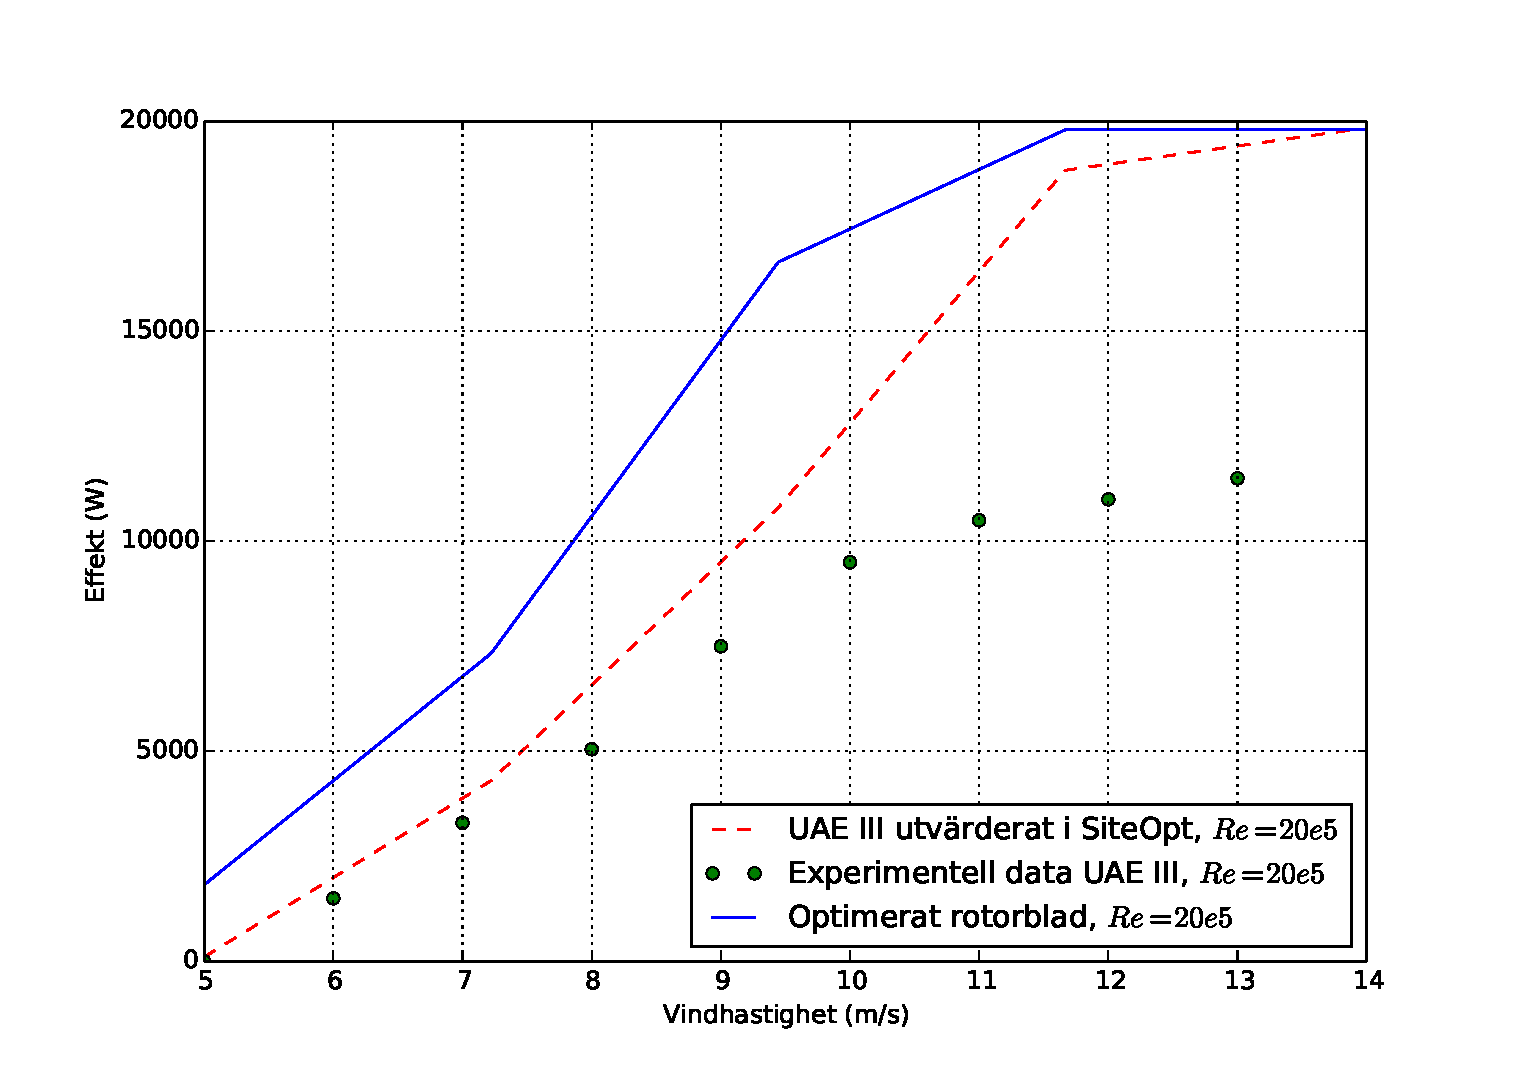
\includegraphics[width=1\textwidth]{powercurvecompare}
  \caption{Effektkurvor för referensfallet UAE III och det optimerade rotorbladet.}
  \label{powercurvecompare}
\end{figure}

Effektkurvan för det rotorbladet som optimeringen tagit fram ses i \fref{powercurvecompare}. Notera att SiteOpts utvärderade effektkurva avviker lite från den i \ref{mattstocksfall} eftersom denna endast är utvärderad vid $Re = 20\times10^5$.

Vingprofilen som optimeringen tagit fram visas i \fref{AFjamforelse} tillsammans med utgångspunkten S809 för jämförelse och är alltså samma för hela rotorbladet. 

\begin{figure}[!h]
  \centering
  \includegraphics[width=1\textwidth]{AFjamforelse}
  \caption{Den optimerade vingprofilen jämfört med ursprungsprofilen S809.}
  \label{AFjamforelse}
\end{figure}

I \fref{kordatwistjamforelse} syns hur korda- och twistdistribution skiljer sig från utgångspunkten UAE III. 

\begin{figure}[!h]
  \centering
  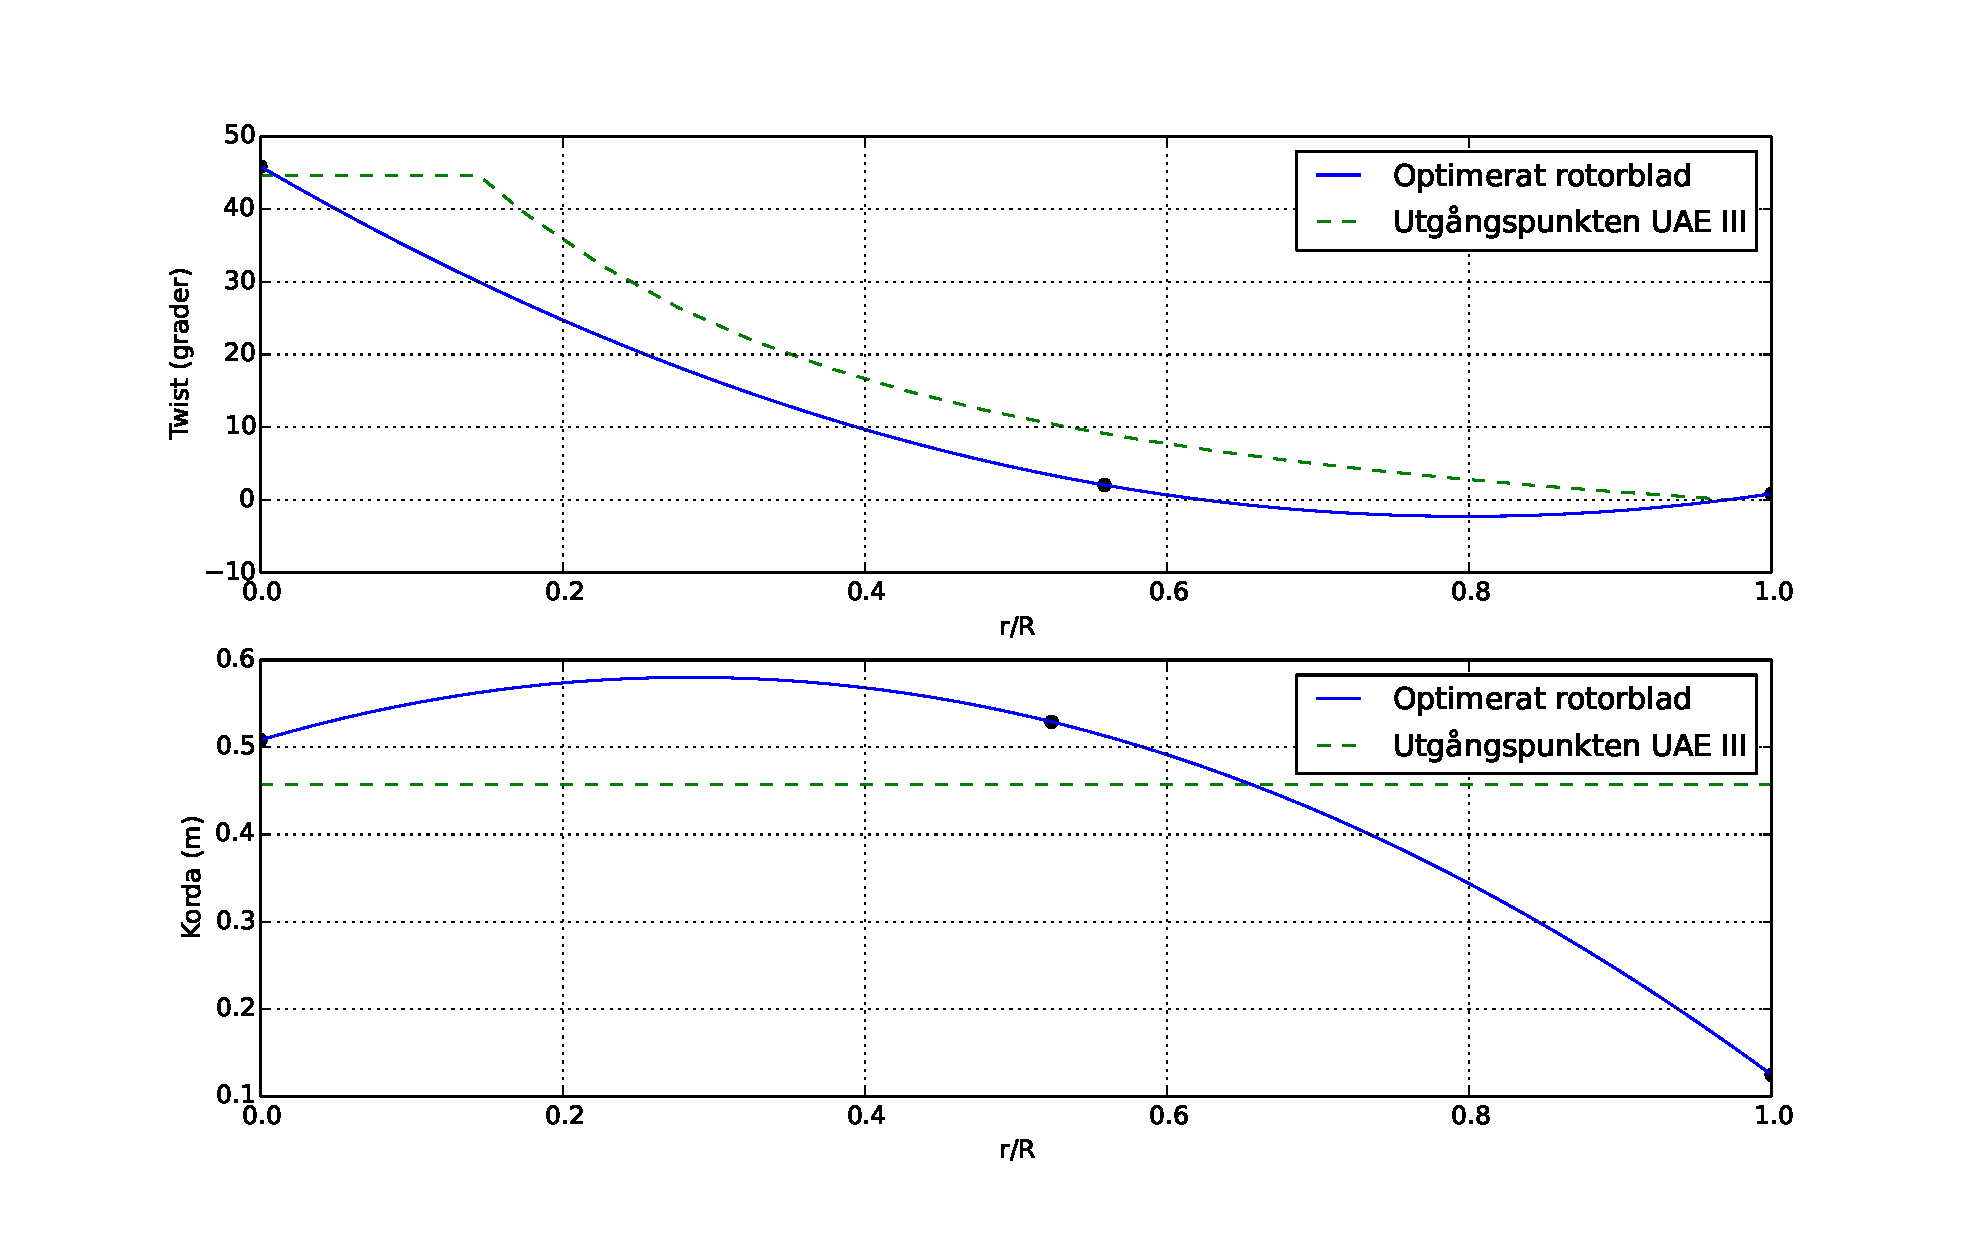
\includegraphics[width=1\textwidth]{kordatwistjamforelse}
  \caption{Det optimerade rotorbladets korda- och twistdistribution jämfört med utgångspunkten UAE III.}
  \label{kordatwistjamforelse}
\end{figure}

I \fref{Cljamforelse} och \fref{Cdjamforelse} presenteras lyft- och motståndskoefficientdata för den optimerade vingprofilen i jämförelse med datan \textsc{Xfoil} ger för S809. Även experimentell data för S809 har inhämtats från \citet{s809re20}. Detta ger en indikation på hur mycket \textsc{Xfoil} överskattar lyft- och motståndskoefficienter vid högre $\alpha$ vilket framkom i litteraturstudien. Detta  bör tas i beaktande när den optimerade vingprofilens data studeras.

\begin{figure}[!htb]
  \centering
  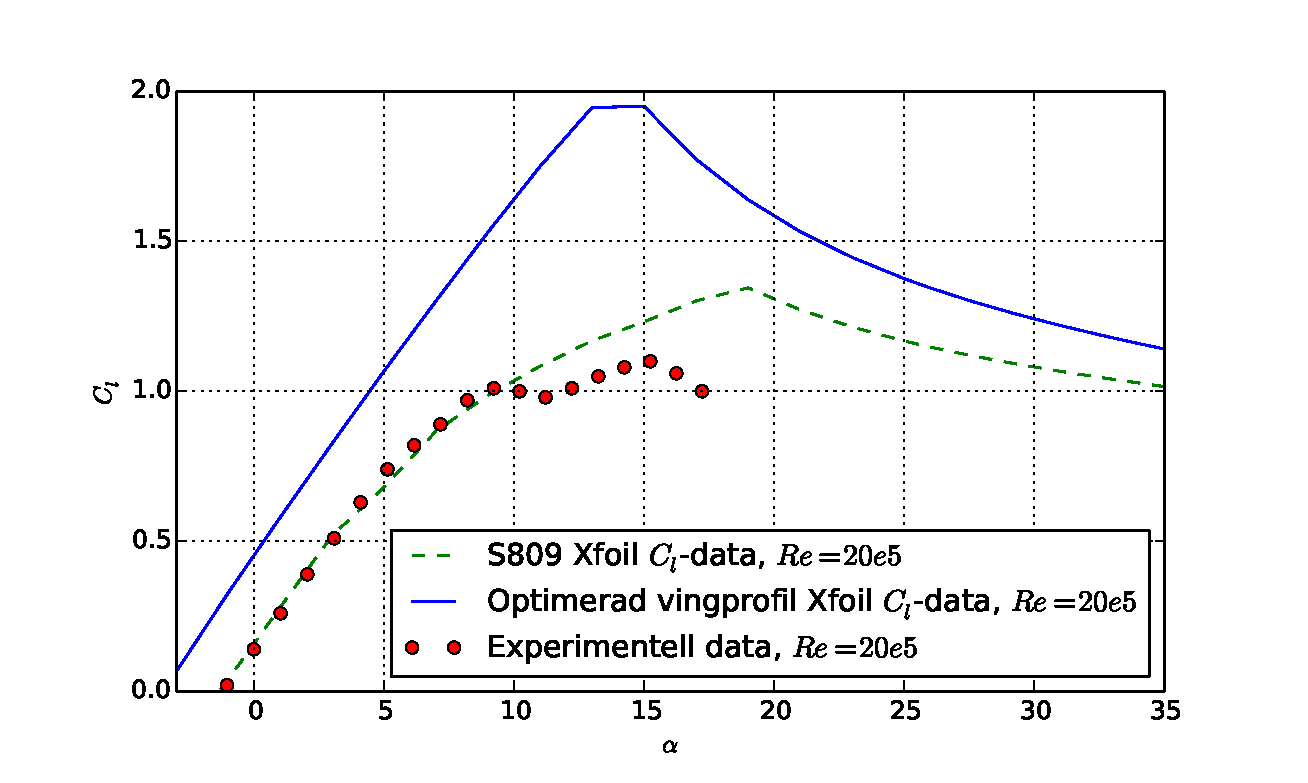
\includegraphics[width=1\textwidth]{Cljamforelse}
  \caption{Lyftkoefficient för den optimerade vingprofilen och utgångspunkten S809 utvärderat i \textsc{Xfoil} samt experimentell data för S809 från \citet{s809re20}.}
  \label{Cljamforelse}
\end{figure}

\begin{figure}[!htb]
  \centering
  \includegraphics[width=1\textwidth]{Cdjamforelse}
  \caption{Motståndskoefficient för den optimerade vingprofilen och utgångspunkten S809 utvärderat i \textsc{Xfoil}.}
  \label{Cdjamforelse}
\end{figure}

